\section{Kernels}
\smallskip \hrule height 2pt \smallskip
If the data is not linearly separable and/or you want a wiggly boundary, use kernels. 

Can give you nonlinear boundaries (good) but the feature space can get really large really quickly. 

Example mapping of data that is not linearly separable to a separable higher dimension space: \hfill \\
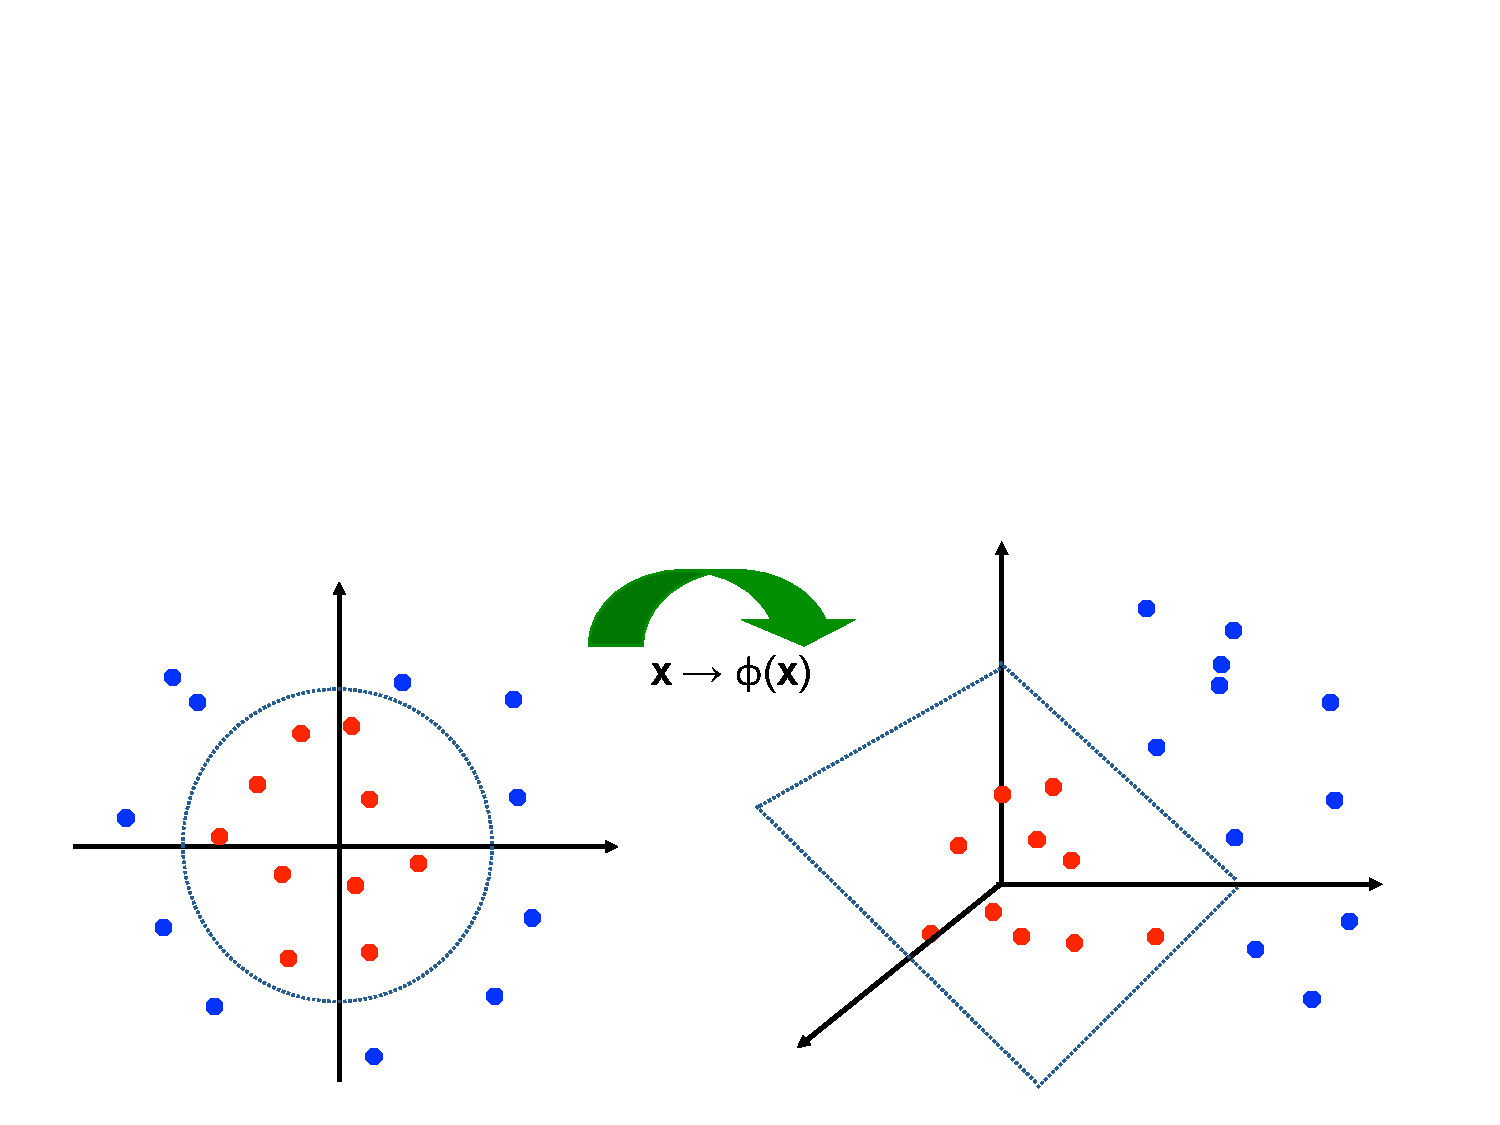
\includegraphics[width=2.5in]{figures/example_kernel_separation.pdf}  \hfill \\

General idea: \hfill \\
If $\bm{x}$ is in $R^n$, then $\phi(\bm{x})$ is in $R^m$ for $m>n$. \hfill \\
We can now learn feature weights $\bm{w}$ in $R^m$ and predict using $y = sign(\bm{w} \cdot \phi(\bm{x}))$. \hfill \\
\textbf{A linear function in the higher dimensional space will be non-linear in the original space.}  \hfill \\

\subsubsection{Danger of Mapping to a Higher Dimensional Space:}
The number of terms in a polynomial of degree $d$ for $m$ input features is 
$\displaystyle {d + m - 1}\choose{d} $ $ \displaystyle = \frac{d + m - 1}{d!(m-1)!}$. \hfill \\
This grows fast!  For $d=6$, $m=100$ you get about 1.6 billion terms.  \hfill \\

We are taking a dot product of $m$ rows for the feature space times $d$ columns of polynomial. 
But you also have terms for combinations of features.  E.g. 
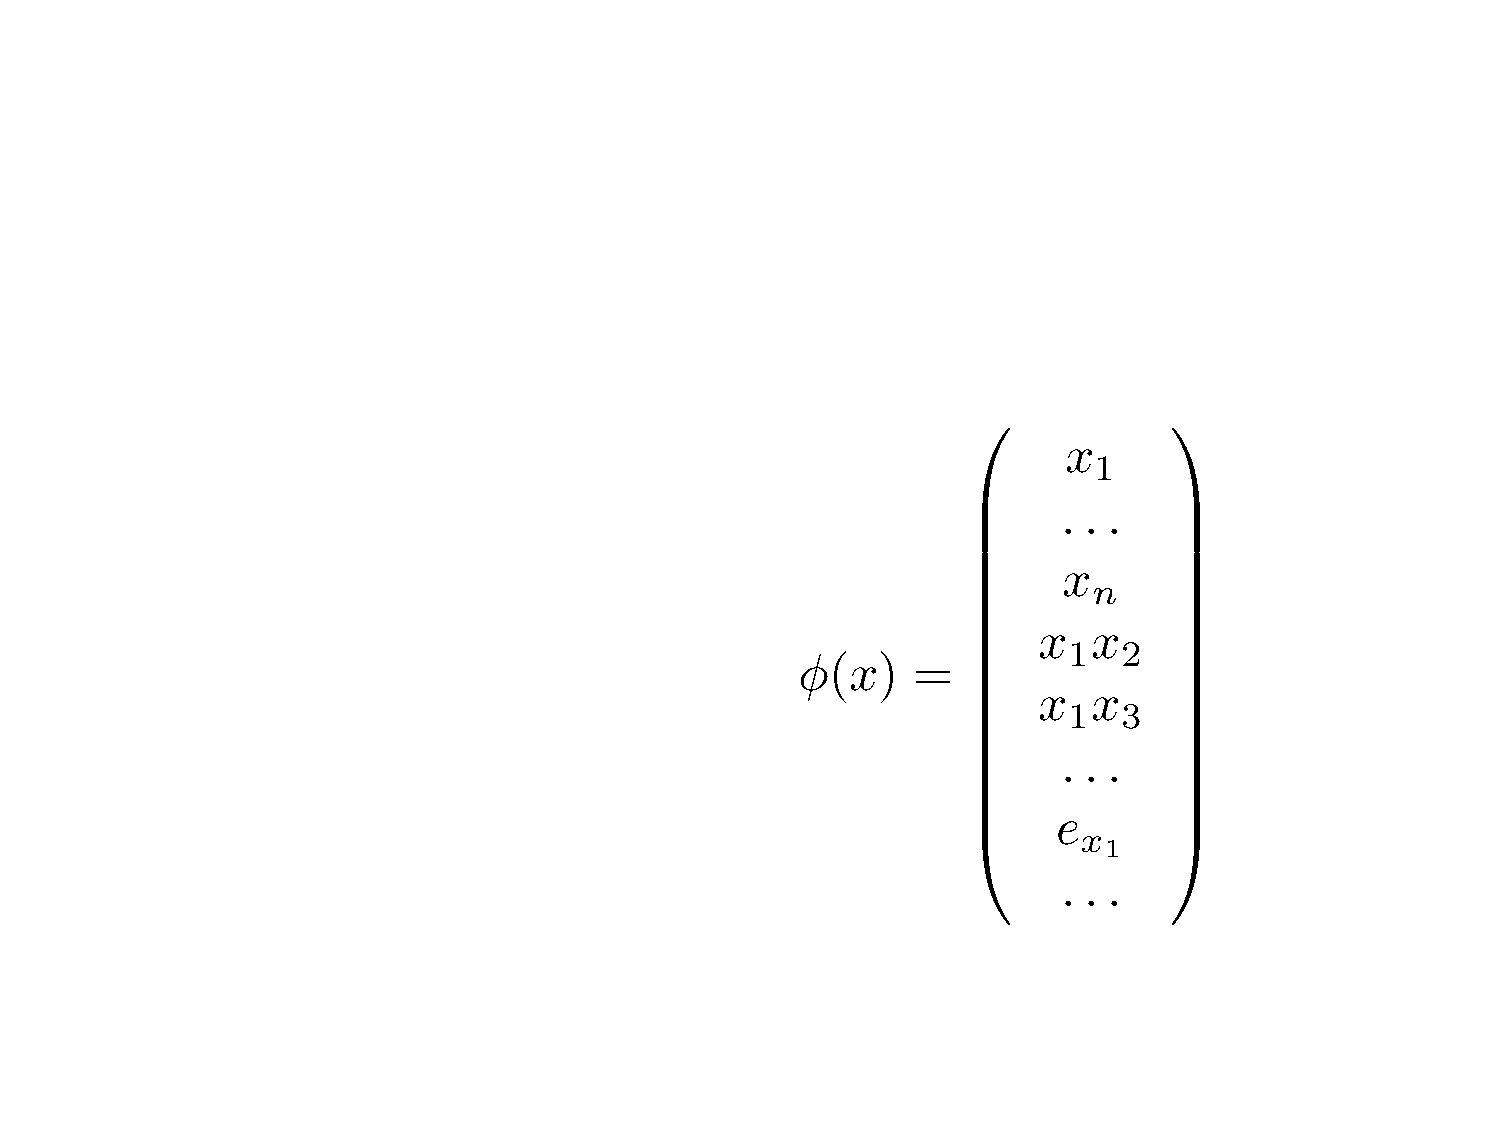
\includegraphics[width=0.8in]{figures/example_kernel.pdf}

\subsubsection{Efficient dot-product of polynomials}
For polynomials of degree exactly $d$, the dot product in higher dimensional space can be written as a dot product in lower dimensional space.  \hfill \\
For $m=2$ (2 features): \hfill \\
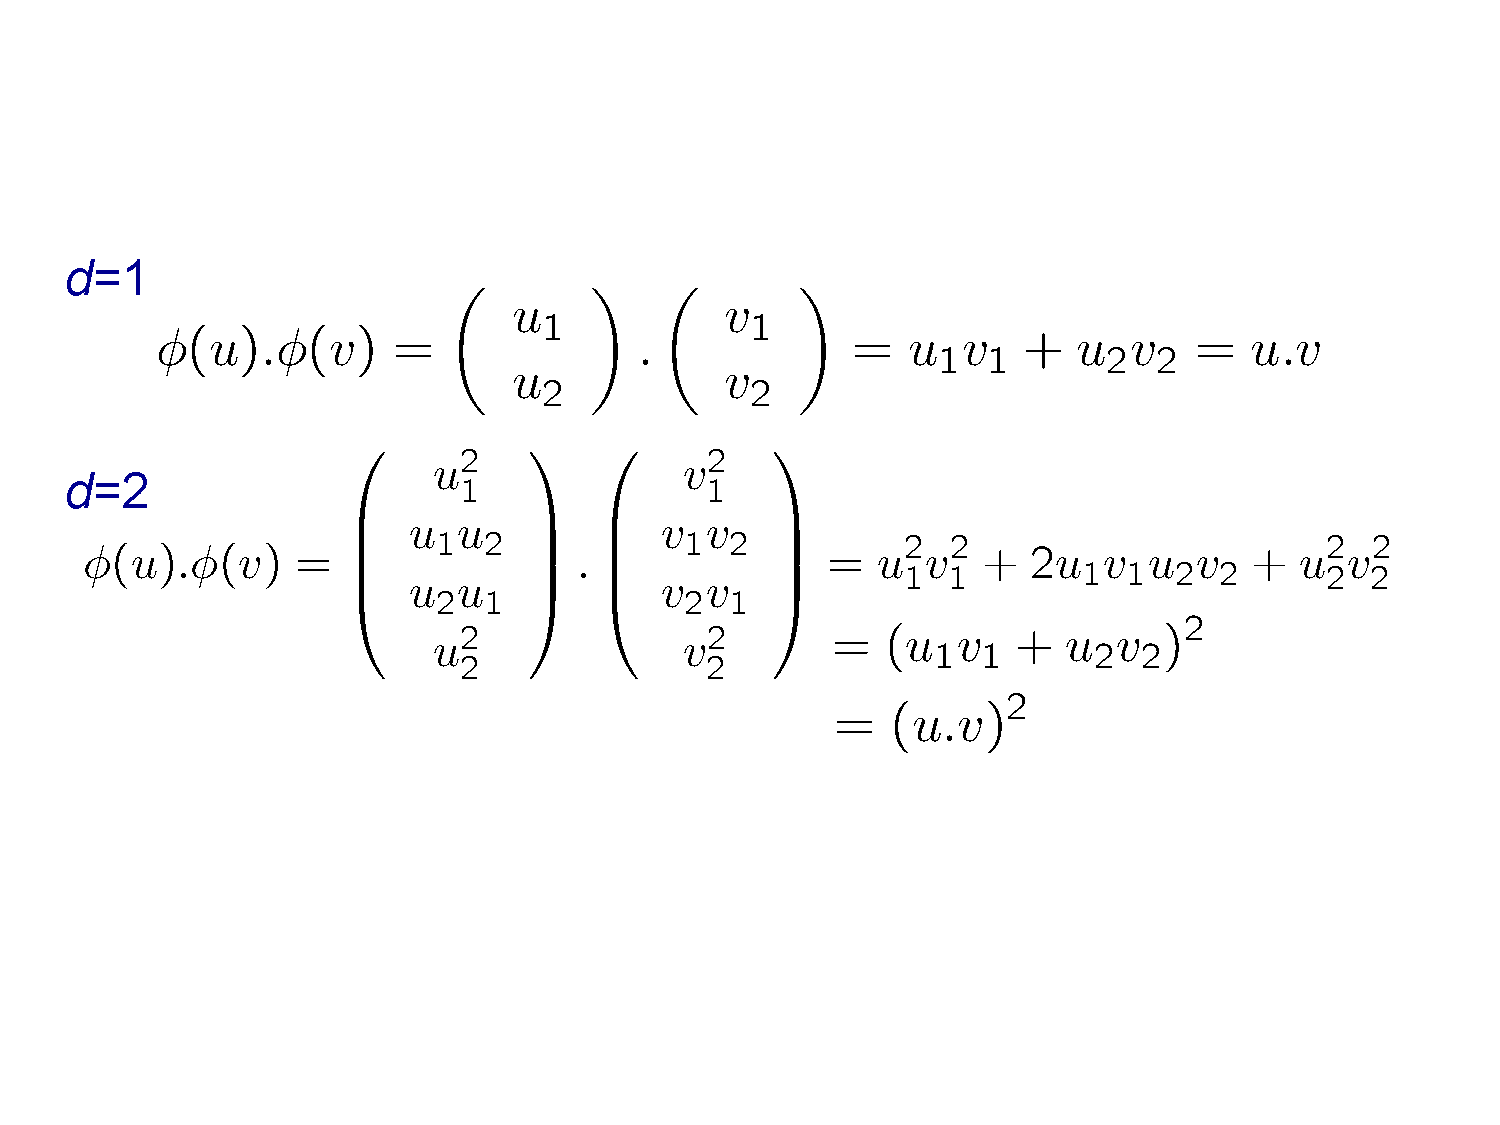
\includegraphics[width=2.5in]{figures/kernel_dot_polynomials.pdf}  \hfill \\
note: here the $.$ is a dot product, not horizontal space fill like a previous lecture. \hfill \\
$u_1$ is feature 1's value, and $u_2$ is feature 2's value. \hfill \\
Polynomial of exactly degree $d$ means we \underline{don't} have a constant bias term like in homework 3 with $[1, \sqrt{2}u, u^2]$  \hfill \\
This is just factoring.  \hfill \\
\hfill \\

Proof not shown, but for any $d$: \hfill \\
$K(u, v) = \bm{\phi}(u).\bm{\phi}(v) = (u.v)^d$

\subsection{The "Kernel Trick"}
A \textbf{kernel function} defines a dot product in some feature space: 
\begin{align*}
	K(\bm{u}, \bm{v}) =\bm{\phi}(\bm{u}) \cdot \bm{\phi}(\bm{v})
\end{align*}
Where $\bm{u}$, $\bm{v}$ are points in your training or test set, each with their own features. \hfill \\ 
Or $\bm{u}$ could be a data point and $\bm{v}$ could be the $\bm{w}$ of the hyperplane that you need to dot against to classify new points.
 \hfill \\
 
 If $\bm{u}$, $\bm{v}$ each have two dimensions (2 features): \hfill \\

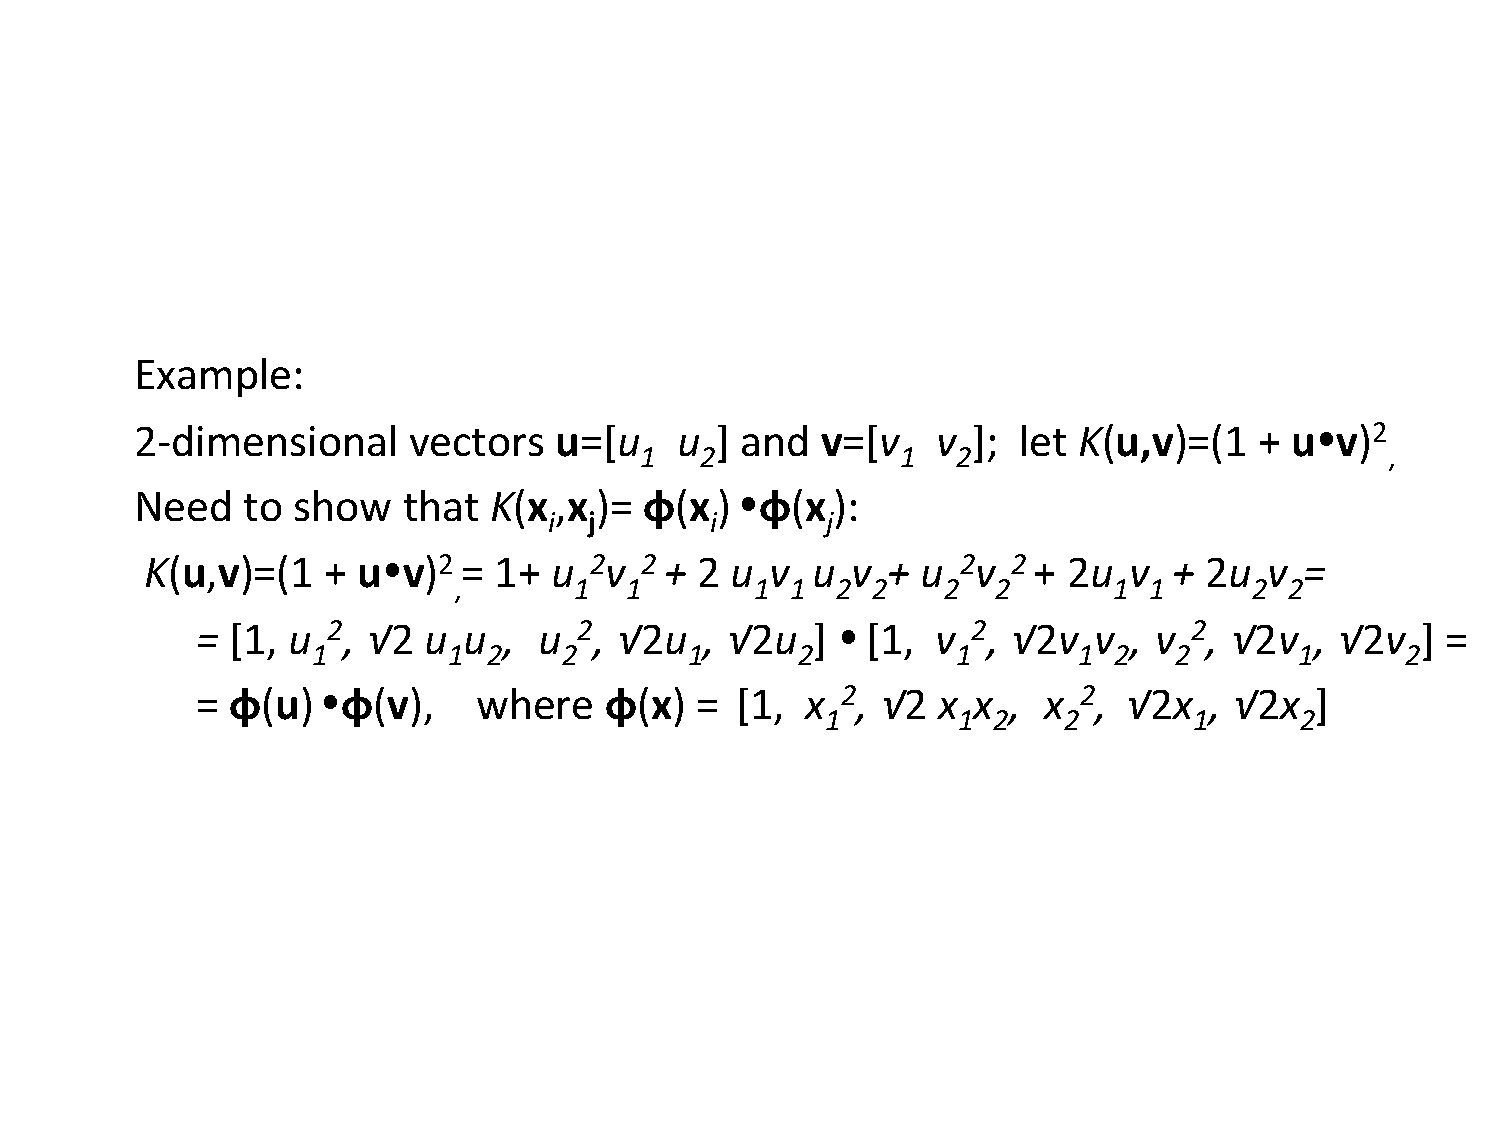
\includegraphics[width=3.1in]{figures/example_kernel_math.pdf} \hfill \\
Thus, a kernel function \textit{implicitly} maps data to a high-dimensional space without the need to compute each $\bm{\phi}(\bm{x})$ explicitly.   \hfill \\
 \hfill \\

Translation for this particular kernel: \hfill \\
We want to get the perks of the high dimensional space given by $\bm{\phi}(\bm{x}) = [1, x_1^2, \sqrt{2}x_1 x_2, x_2^2, \sqrt{2} x_1, \sqrt{2} x_2]$ where $\bm{x}$ is either $\bm{u}$ or $\bm{v}$.  \hfill \\
But this is computationally expensive because there are many terms in that thing.  \hfill \\
If we take the dot product of two vectors $\bm{\phi}(\bm{u})$, $\bm{\phi}(\bm{v})$ we get some magic: \hfill \\
\begin{align*}
	\bm{\phi}(\bm{u}) \cdot \bm{\phi}(\bm{v}) &= [1, u_1^2, \sqrt{2}u_1 u_2, u_2^2, \sqrt{2} u_1, \sqrt{2} u_2]  \cdot \quad \mbox{(line wrapped)} \\
			& \quad \quad [1, v_1^2, \sqrt{2}v_1 v_2, v_2^2, \sqrt{2} v_1, \sqrt{2} v_2]   \\
		&=  (1 + \bm{u} \cdot \bm{v})^2
\end{align*}
Can do $(1 + \bm{u} \cdot \bm{v})^2$ with a dot product that only includes multiplying $[u_1, u_2]^T[v_1, v_2]$.     \hfill \\ 
That's a lot less computation/memory expensive than the full dot product above.  \hfill \\
If that leads to good separation, you are a happy machine learner!   \hfill \\
\textbf{This is true for other kernels in general.}   \hfill \\
($(1 + \bm{u} \cdot \bm{v})^2$ would take other forms for other cases).   \hfill \\
\hfill \\

It is essential that everything you want to do with your transformed vectors is representable by simple dot products.
If you can't simplify it down to dot products of the original vector then there's no point. 





